\begin{figure}[H]
    \centering
    % --- Escenario A ---
    \begin{subfigure}[b]{0.45\textwidth}
        \centering
		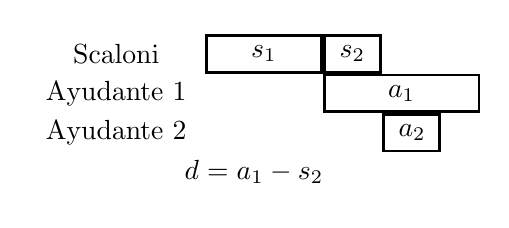
\begin{tikzpicture}
	% Paths, nodes and wires:
	\node[shape=rectangle, draw, line width=1pt, minimum width=1.465cm, minimum height=0.465cm] at (1.75, 5.75){} node[anchor=center, align=center, text width=1.077cm, inner sep=6pt] at (1.75, 5.75){$s_1$};
	\node[shape=rectangle, draw, line width=1pt, minimum width=0.715cm, minimum height=0.465cm] at (2.875, 5.75){} node[anchor=center, align=center, text width=0.327cm, inner sep=6pt] at (2.875, 5.75){$s_2$};
	\node[shape=rectangle, draw, line width=1pt, minimum width=1.965cm, minimum height=0.465cm] at (3.5, 5.25){} node[anchor=center, align=center, text width=1.577cm, inner sep=6pt] at (3.5, 5.25){$a_1$};
	\node[shape=rectangle, draw, line width=1pt, minimum width=0.715cm, minimum height=0.465cm] at (3.625, 4.75){} node[anchor=center, align=center, text width=0.327cm, inner sep=6pt] at (3.625, 4.75){$a_2$};
	\node[shape=rectangle, minimum width=2.215cm, minimum height=0.465cm] at (-0.125, 5.75){} node[anchor=center, align=center, text width=1.827cm, inner sep=6pt] at (-0.125, 5.75){Scaloni};
	\node[shape=rectangle, minimum width=2.215cm, minimum height=0.465cm] at (-0.125, 5.25){} node[anchor=center, align=center, text width=1.827cm, inner sep=6pt] at (-0.125, 5.25){Ayudante 1};
	\node[shape=rectangle, minimum width=2.215cm, minimum height=0.465cm] at (-0.125, 4.75){} node[anchor=center, align=center, text width=1.827cm, inner sep=6pt] at (-0.125, 4.75){Ayudante 2};
	\node[shape=rectangle, minimum width=2.215cm, minimum height=0.465cm] at (1.625, 4.25){} node[anchor=center, align=center, text width=1.827cm, inner sep=6pt] at (1.625, 4.25){$d = a_1-s_2$};
\end{tikzpicture}
        \caption{Caso en donde $a_1$ mismo tiempo que $a_2$}
    \end{subfigure}
    \hfill
    % --- Escenario B ---
    \begin{subfigure}[b]{0.45\textwidth}
        \centering
		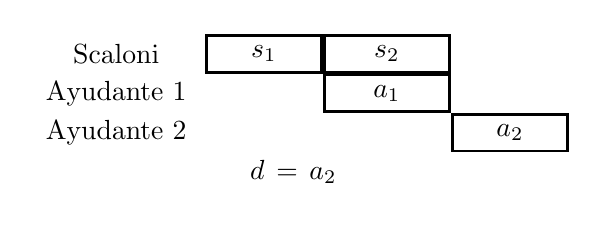
\begin{tikzpicture}
	% Paths, nodes and wires:
	\node[shape=rectangle, draw, line width=1pt, minimum width=1.465cm, minimum height=0.465cm] at (8.688, 5.75){} node[anchor=center, align=center, text width=1.077cm, inner sep=6pt] at (8.688, 5.75){$s_1$};
	\node[shape=rectangle, draw, line width=1pt, minimum width=1.59cm, minimum height=0.465cm] at (10.25, 5.75){} node[anchor=center, align=center, text width=1.202cm, inner sep=6pt] at (10.25, 5.75){$s_2$};
	\node[shape=rectangle, draw, line width=1pt, minimum width=1.59cm, minimum height=0.465cm] at (10.25, 5.25){} node[anchor=center, align=center, text width=1.202cm, inner sep=6pt] at (10.25, 5.25){$a_1$};
	\node[shape=rectangle, draw, line width=1pt, minimum width=1.465cm, minimum height=0.465cm] at (11.813, 4.75){} node[anchor=center, align=center, text width=1.077cm, inner sep=6pt] at (11.813, 4.75){$a_2$};
	\node[shape=rectangle, minimum width=2.215cm, minimum height=0.465cm] at (6.813, 5.75){} node[anchor=center, align=center, text width=1.827cm, inner sep=6pt] at (6.813, 5.75){Scaloni};
	\node[shape=rectangle, minimum width=2.215cm, minimum height=0.465cm] at (6.813, 5.25){} node[anchor=center, align=center, text width=1.827cm, inner sep=6pt] at (6.813, 5.25){Ayudante 1};
	\node[shape=rectangle, minimum width=2.215cm, minimum height=0.465cm] at (6.813, 4.75){} node[anchor=center, align=center, text width=1.827cm, inner sep=6pt] at (6.813, 4.75){Ayudante 2};
	\node[shape=rectangle, minimum width=2.215cm, minimum height=0.465cm] at (9.063, 4.25){} node[anchor=center, align=center, text width=1.827cm, inner sep=6pt] at (9.063, 4.25){$d =a_2$};
\end{tikzpicture}
        \caption{Caso en donde $a_1$ menor tiempo de $a_2$}
    \end{subfigure}

    \vspace{1cm} % Espacio entre filas

    % --- Escenario C ---
    \begin{subfigure}[b]{0.45\textwidth}
        \centering
        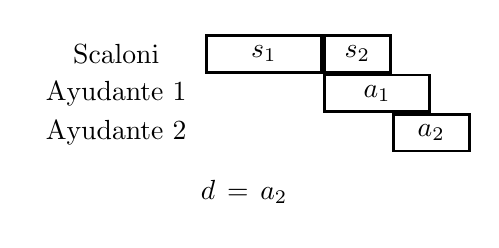
\begin{tikzpicture}
	% Paths, nodes and wires:
	\node[shape=rectangle, draw, line width=1pt, minimum width=1.465cm, minimum height=0.465cm] at (2.125, 1.75){} node[anchor=center, align=center, text width=1.077cm, inner sep=6pt] at (2.125, 1.75){$s_1$};
	\node[shape=rectangle, draw, line width=1pt, minimum width=0.84cm, minimum height=0.465cm] at (3.313, 1.75){} node[anchor=center, align=center, text width=0.452cm, inner sep=6pt] at (3.313, 1.75){$s_2$};
	\node[shape=rectangle, draw, line width=1pt, minimum width=1.34cm, minimum height=0.465cm] at (3.563, 1.25){} node[anchor=center, align=center, text width=0.952cm, inner sep=6pt] at (3.563, 1.25){$a_1$};
	\node[shape=rectangle, draw, line width=1pt, minimum width=0.965cm, minimum height=0.465cm] at (4.25, 0.75){} node[anchor=center, align=center, text width=0.577cm, inner sep=6pt] at (4.25, 0.75){$a_2$};
	\node[shape=rectangle, minimum width=2.215cm, minimum height=0.465cm] at (0.25, 1.75){} node[anchor=center, align=center, text width=1.827cm, inner sep=6pt] at (0.25, 1.75){Scaloni};
	\node[shape=rectangle, minimum width=2.215cm, minimum height=0.465cm] at (0.25, 1.25){} node[anchor=center, align=center, text width=1.827cm, inner sep=6pt] at (0.25, 1.25){Ayudante 1};
	\node[shape=rectangle, minimum width=2.215cm, minimum height=0.465cm] at (0.25, 0.75){} node[anchor=center, align=center, text width=1.827cm, inner sep=6pt] at (0.25, 0.75){Ayudante 2};
	\node[shape=rectangle, minimum width=2.215cm, minimum height=0.465cm] at (1.875, -0){} node[anchor=center, align=center, text width=1.827cm, inner sep=6pt] at (1.875, -0){ $d = a_2$};
\end{tikzpicture}
        \caption{Caso en donde $a_1$  de $a_2$}
    \end{subfigure}
    \hfill
    % --- Escenario D ---
    \begin{subfigure}[b]{0.45\textwidth}
        \centering
        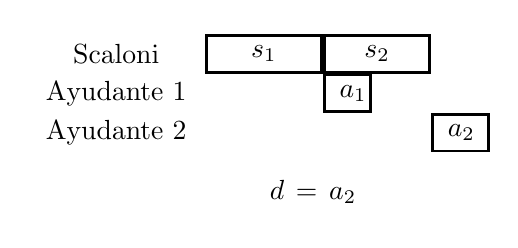
\begin{tikzpicture}
	% Paths, nodes and wires:
	\node[shape=rectangle, draw, line width=1pt, minimum width=1.465cm, minimum height=0.465cm] at (8.625, 1.75){} node[anchor=center, align=center, text width=1.077cm, inner sep=6pt] at (8.625, 1.75){$s_1$};
	\node[shape=rectangle, draw, line width=1pt, minimum width=1.34cm, minimum height=0.465cm] at (10.063, 1.75){} node[anchor=center, align=center, text width=0.952cm, inner sep=6pt] at (10.063, 1.75){$s_2$};
	\node[shape=rectangle, draw, line width=1pt, minimum width=0.59cm, minimum height=0.465cm] at (9.688, 1.25){} node[anchor=center, align=center, text width=0.202cm, inner sep=6pt] at (9.688, 1.25){$a_1$};
	\node[shape=rectangle, draw, line width=1pt, minimum width=0.715cm, minimum height=0.465cm] at (11.125, 0.75){} node[anchor=center, align=center, text width=0.327cm, inner sep=6pt] at (11.125, 0.75){$a_2$};
	\node[shape=rectangle, minimum width=2.215cm, minimum height=0.465cm] at (6.75, 1.75){} node[anchor=center, align=center, text width=1.827cm, inner sep=6pt] at (6.75, 1.75){Scaloni};
	\node[shape=rectangle, minimum width=2.215cm, minimum height=0.465cm] at (6.75, 1.25){} node[anchor=center, align=center, text width=1.827cm, inner sep=6pt] at (6.75, 1.25){Ayudante 1};
	\node[shape=rectangle, minimum width=2.215cm, minimum height=0.465cm] at (6.75, 0.75){} node[anchor=center, align=center, text width=1.827cm, inner sep=6pt] at (6.75, 0.75){Ayudante 2};
	\node[shape=rectangle, minimum width=2.215cm, minimum height=0.465cm] at (9.25, -0){} node[anchor=center, align=center, text width=1.827cm, inner sep=6pt] at (9.25, -0){$d = a_2$};
\end{tikzpicture}
        \caption{Caso en donde $a_1$ termina después de $a_2$}
    \end{subfigure}

    \caption{Análisis con tiempos con 2 rivales.}
    \label{fig:escenarios_posibles}
\end{figure}
